\section{Architecture}
\label{SEC:architecture}

\begin{figure}
  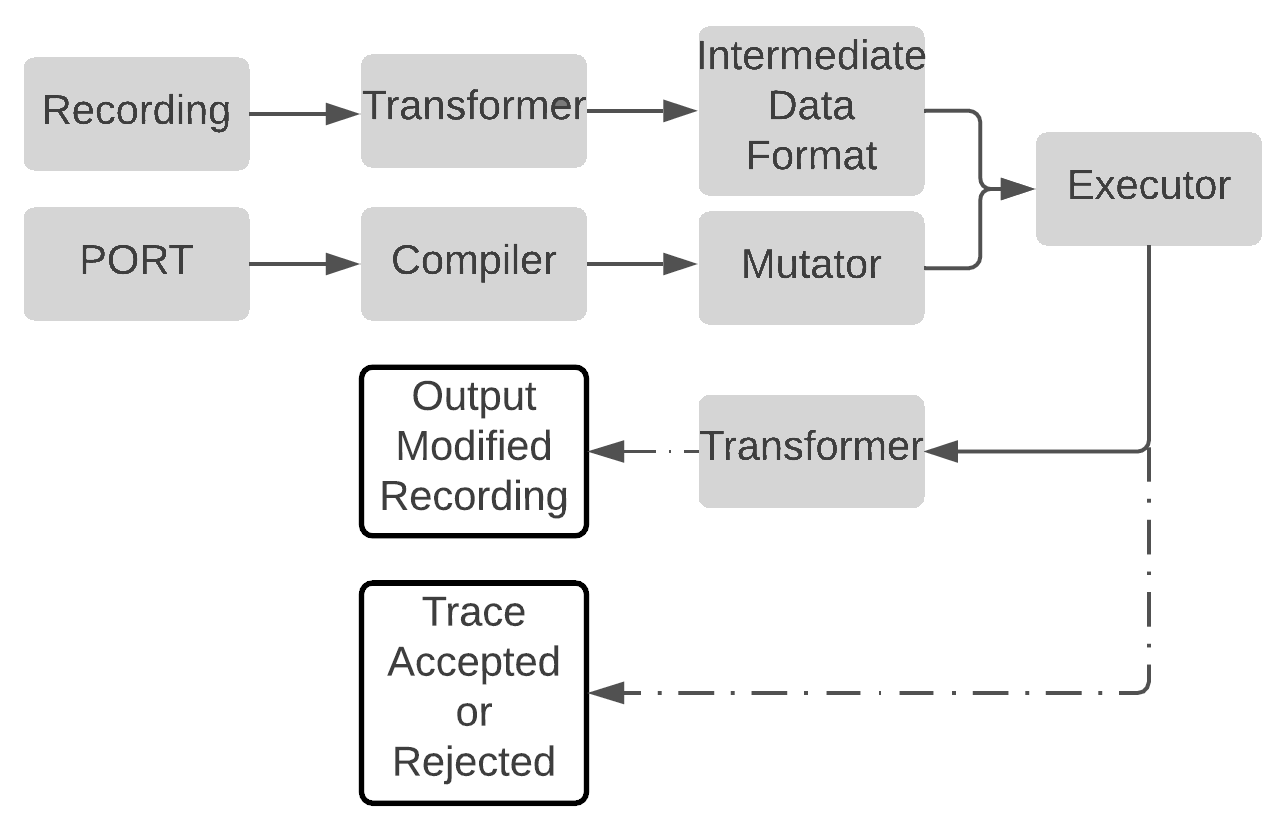
\includegraphics[scale=.08, frame]{images/architecture}
  \caption{The CSlang compiler produces a transducer that operates over a
  generic intermediate representation of the contents of a given trace.}
  \label{fig:architecture}
\end{figure}


The SEA technique's power comes from its ability to capture and encode
anomalies so they can be repeatedly employed in testing applications.  We
reasoned that we could see the most value for our efforts by focusing our
enhancements in this area.  We examined the encoded anomalies used in the
earlier SEA work and found several deficiencies.
They were
long (in terms of lines of code),
difficult to understand,
and tightly coupled to the implementation details of system calls.
We decided to address each of these concerns by developing a new
programming language, CSlang.  Our goal with CSlang was to provide a way to
describe anomalies that was concise, easy to understand, and generic enough
that it could support many message formats.

While the CSlang language is the star of the show, achieving this goal
required several new components.  We found it is best to have an
understanding of these components before diving into the details of the
language itself.
At the core of our improvements is
a new model for recognizing and transforming streams of messages.  Our
model is based on a finite-state transducer and builds upon the earlier SEA
work's success at describing simulation opportunities using deterministic
finite automata.  We chose the transducer as our foundation so that
recognition and transformation of streams could be done at the same time.
This model is generated by compiling a CSlang anomaly description using the
CSlang compiler.

The model doesn't serve much purpose by itself.  It needs a stream of
messages to operate on.  This stream is provided by our second component,
the message format adaptor.
The function of this element is to take a
stream of messages in their in their original representation and convert
them into a format that a CSlang transducer can consume. This conversion process
captures the identifying information and parameters of each message in the
input stream and stores them in CSlang's Intermediate Data Format (IDF).
Operating on this generic intermediate format means CSlang transducers are
not dependent on a specific message format.

%This is important because it
%breaks the system-call dependence of the previous SEA work allowing

%% which helps us achieve our third goal and
Both of the compiled transducer and the converted message stream 
are provided to the CSlang executor.
This program is responsible for passing each message of the stream
to the transducer
so that it may advance its internal state and
produce appropriate output.
This output comes in the form of modifications to the IDF stream itself.
After execution completes a decision is made based on the ending state of
the transducer.  If it is in an accepting state, the stream of messages has
been modified to include an anomaly and will be output in its original
representation.  If the automaton is not in an accepting state, the stream
did not contain an opportunity to simulate the described anomaly.

<Something Something Something how simulation works goes here?>

%\begin{itemize}
%  \item{Language describing anomalies}
%  \item{Formal model of transducer that can implement anomalies}
%  \item{Tool to compile description into said formal transducer}
%  \item{Format-agnostic intermediate data structure (IDS) over which transducer
%  operates}
%  \item{Translation layer for converting to and from concrete data into IDS}
%\end{itemize}

